\subsection{Results}
\label{sec:stretching_constraint_controller_results}

Our goal for this new controller is formulating a set of constraints for the controller to mitigate collision and excessive stretching issues. As mentioned in previous sections, our benchmark controller is based on \cite{Berenson2013} and described in Sec.~\ref{sec:stretching_avoidance_controller}. To evaluate our method we perform experiments in simulation and on a physical robot. The simulator used is Bullet physics \cite{Coumans2010}, however, we emphasize that our method has no knowledge of the simulation parameters or simulation methods used therein. The simulator is used as a ``black-box,'' mainly to stand in for a perception system and to allow us to do repeatable experiments. The physical robot consists of two KUKA iiwa 7DoF arms with Robotiq 3-finger hands.

\todoin{Separate text/wording etc. for model vs controller.}

We ran experiments with scenarios involving both cloth and rope. The parameters are set as $\drkdir = 4$, $\drkdist = 10$, $\drkrot = 20$ for the new model, $l_c = 0.023$, and $s_s = 0.4$ for the new controller. The parameters we used for the benchmark method are its default best value found in \cite{McConachie2018}. The stretching detection ratio is set as $\stretchmax = 1.667$ for the cloth and $\stretchmax = 1.1$ for the rope. The maximum gripper motion is set as $grippervelmaxservo = 0.2$. For the experiment with a task goal defined, a precalculated Dijkstra field for the task will generate the $\deformvel_e$ for each point at each state to move the object toward the goal given each point's current position in the space as described in Sec.~\ref{sec:reducing_error}. All experiments were run on a i7-8700K 3.7 GHz CPU with 32 GB of RAM. A video showing the experiments is included with this paper.


\subsection{Constraint Enforcement}
\label{Results: Object Stretching Avoidance}

Since the benchmark controller can already handle the collision constraint very well, and the new controller addresses the collision constraint in the similar way as the benchmark, there is not a significant difference in how the collision constraint is enforced. However, the stretching constraint shows a very clear improvement.

The metrics of stretching avoidance is the stretching ratio $\stretchcurr$ defined in Section \ref{Method_Overstretch}. A controller with good stretching avoidance should prevent $\stretchcurr$ from increasing beyong a certain threshold.

The two experiments we used for the stretching avoidance test are the rope-wrapping-cylinder and the cloth-passing-single-pole, shown in Fig.\ref{fig:experimental_setup_scene} (left column). We ran each controller separately for a fixed amount of time for each task and show $\stretchcurr$ vs. time for both controllers in Fig. \ref{fig:experiment_stretching_factorFig: experiment_stretching_factor}. In both these two setups, the desired object motion $\deformvel_e$ generated by the Dijkstra field will tear the object unless overstretching is prevented.%, thus the 

Fig. \ref{fig:experiment_stretching_factorFig: experiment_stretching_factor} shows the new controller is able to prevent further stretching happening when the object is taut for both the rope and the cloth. In the rope test, the new controller can prevent overstretching with $s_s = 0.4$, as defined in Eq.\ref{Eq: Stretching_avoidance_Method_This_Paper}. We can see the $\stretchcurr$ of the benchmark methods keeps growing beyond this threshold, while the $\stretchcurr$ of the new method stays close to the threshold. In the cloth test, the benchmark method's $\stretchcurr$ (in purple) increases above the threshold $\stretchmax = 1.667$ for cloth, and a sudden drop in $\stretchcurr$ happens after running the test for $2$ seconds. This drop is the ``tearing'' point in the simulator. Though we still see overstretching happened using the new method for some settings of $s_s$, in all cases the $\stretchcurr$ converged before tearing happened (instead of growing without bound). 

\begin{figure}[t]
    \centering
    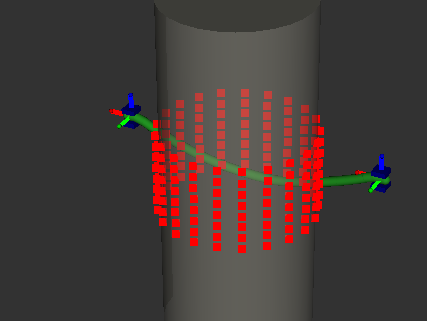
\includegraphics[width=.45\linewidth]{rope_cylinder}\hfill
    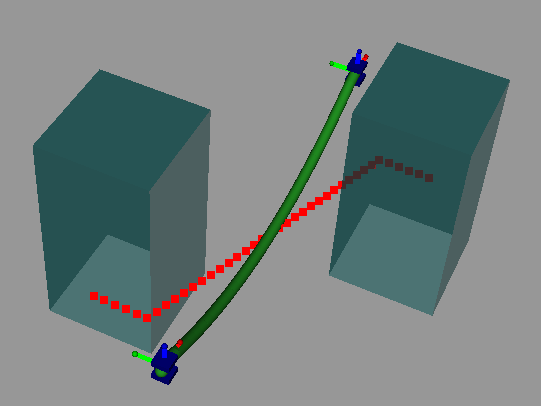
\includegraphics[width=.45\linewidth]{rope_zig_match}\\
    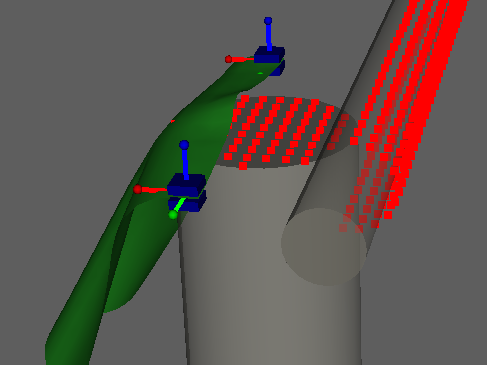
\includegraphics[width=.45\linewidth]{cloth_wafr}\hfill
    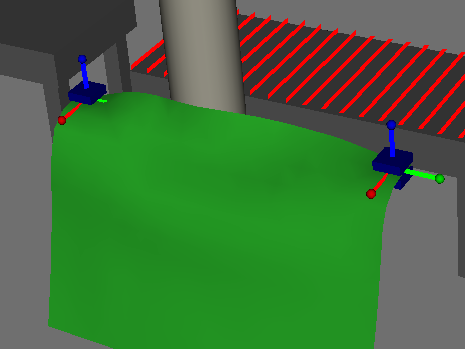
\includegraphics[width=.45\linewidth]{cloth_single_pole}%
    \caption{Initial state of the four experiments, where the red points act as attractors for the deformable object.}
    \label{fig:experimental_setup_scene}
\end{figure}


\begin{figure}[t]
    \centering
    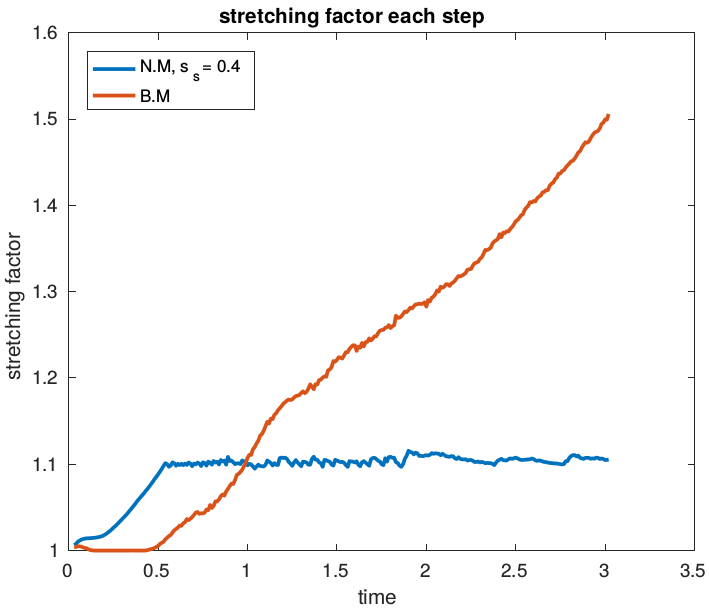
\includegraphics[width=.45\linewidth]{stretching_rope_cylinder} \hfill
    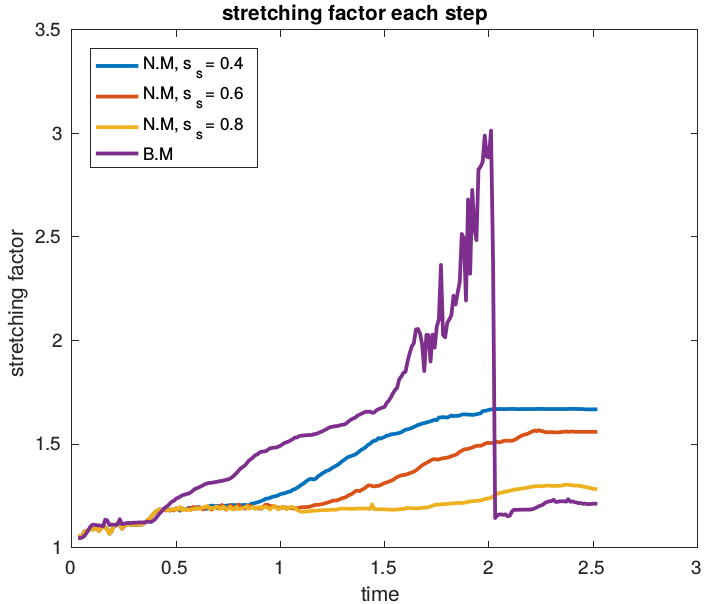
\includegraphics[width=.45\linewidth]{stretching_cloth_single_pole}%
    \caption{Cloth passing single pole}
    \label{Fig: stretching factor scene_cloth_single_pole}
    \caption{(a) The red line shows the $\stretchcurr$ of the benchmark and the blue line shows the $\stretchcurr$ of the new controller with $s_s = 0.4$ throughout the simulation. (b) The purple line shows the $\stretchcurr$ of the benchmark, and the blue, red, and yellow lines each show the $\stretchcurr$ of the new controller with $s_s = 0.4$, $s_s = 0.6$, and $s_s = 0.8$, respectively.}
    \label{fig:experiment_stretching_factorFig: experiment_stretching_factor}
\end{figure}




%We find that setting a tighter constraint, such as increasing the value of $s_s$, can help prevent excessive stretching in the object, as shown in Fig. \ref{Fig: cos_stretching}. 


% Explain the trade-off between constraints avoidance and control accuracy
%Examining Fig. \ref{Fig: experiment_model_error} and Fig. \ref{fig:experiment_stretching_factorFig: experiment_stretching_factor}, we found that when there is no constraints violation detected, the new controller can generally have a smaller control error.
%When the constraints violation happens, the new controller will tend to mitigate this violation and take the trade off in control accuracy.  



\subsection{Controller Task Performance} \label{Results:Controller Task Performance}

Besides the quantitative analysis of the model accuracy and stretching avoidance, we ran another two experiments, rope-matching-zig-path and cloth-covering-two-cylinder, one each with the rope or the cloth, as shown in Fig.~\ref{fig:experimental_setup_scene} to see how the new method performed for some coverage tasks. Both the benchmark and the new controllers are able to perform these tasks with comparable performance; reaching approximately the same configurations when forward progress stops due to a local minimum (Fig.~\ref{fig:cloth_wafr_performance}), and completing the task (Fig.~\ref{fig:zigzeg_performance}). This result suggests that we have not lost functionality with respect to the benchmark despite changing the model and control method used.


\begin{figure}[t]
    \centering
    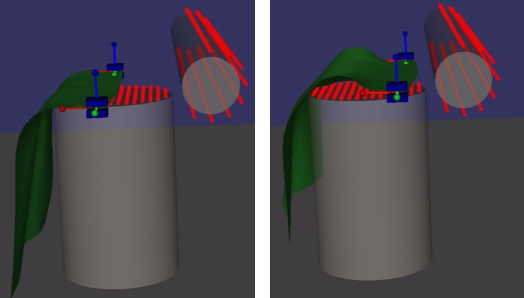
\includegraphics[width=\columnwidth]{cloth_wafr_performance.png}
    \caption{Cloth-covering-two-cylinder task start and end configurations. Both controllers are unable to make progress due to a local minima.}
    \label{fig:cloth_wafr_performance}
\end{figure}


\begin{figure}[t]
    \centering
    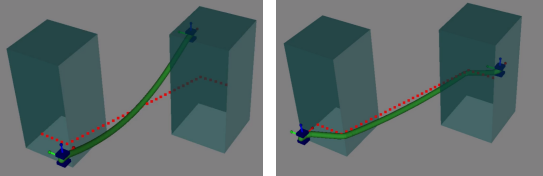
\includegraphics[width=\columnwidth]{zigzeg_performance.png}
    \caption{Rope-matching-zig-path start and end configurations. Both controllers are able to succeed at the task, bringing the rope into alignment with the desired path.}
    \label{fig:zigzeg_performance}
\end{figure}



\subsection{Physical Robot Experiments}

To evaluate our new model and controller on a physical system, we set up an experiment with cloth-like objects manipulated by two 7DoF KUKA iiwa arms (Fig.~\ref{fig:physical_experiment_screenshots_ctl}). To sense the position of the cloth, we use the AprilTags~\cite{olson2011tags} and IAI Kinect2~\cite{iai_kinect2} libraries. The parameters are set as $\drkdir = 4$, $\drkdist = 10$, $\drkrot = 10$ for the new model, $l_c = 0.08$, and $s_s = 0.6$ for the new controller. We set up a task similar to the cloth-passing-single-pole example using a paper towel. For this task, the baseline controller tears the paper towel while the new controller avoids excessive overstretch, instead wrapping around the pole to reach a local minimum.

\begin{figure}[t]
    \centering
    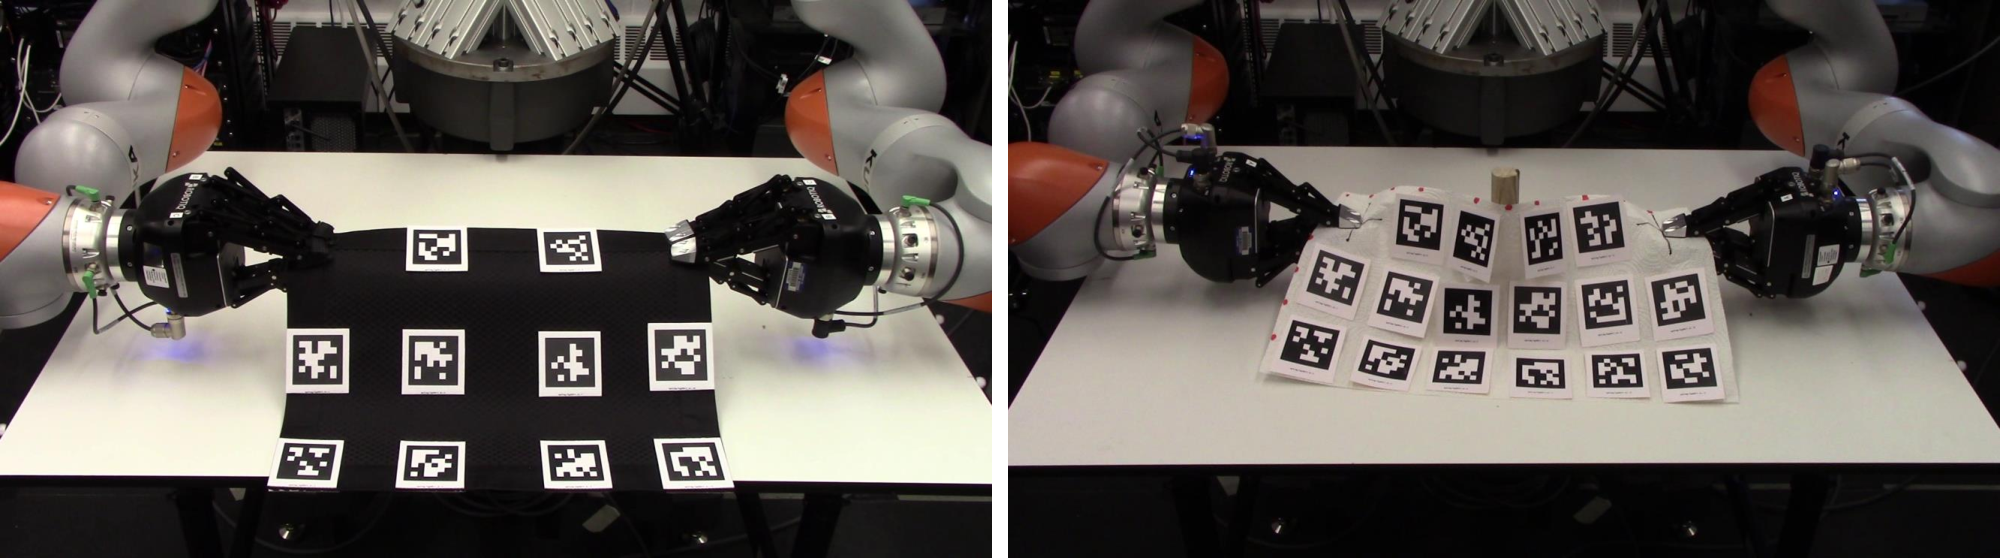
\includegraphics[width=0.85\columnwidth,trim=6.7in 0 0 0,clip]{physical_robot_experiment_screenshots.pdf}
    \caption{Initial setup for the physical robot stretching avoidance test.}
    \label{fig:physical_experiment_screenshots_ctl}
\end{figure}


\subsection{Computation Time}


\begin{table}[t]
%\renewcommand{\arraystretch}{1.2}
\centering
\resizebox{\linewidth}{!}{
\begin{tabular}{|c|c|c|c|c|}
\hline
        & rope-wrapping & rope-matching & cloth-passing & cloth-wrapping \\
        & -cylinder     & -zig-path     & single-pole   & -two-cylinders \\ \hline
BM       & 0.0055   & 0.0054  & 0.0153  & 0.0037   \\ \hline
NM       & 0.0342   & 0.0834  & 0.2363  & 0.1008   \\ \hline
\end{tabular}
}
\caption{Mean computation time (s) to compute the gripper motion for a given state. BM: benchmark method; NM: new method.}
\label{tbl:constraint_controller_time_report}
\end{table}



To verify the practicality of our method, we gathered data comparing its computation time to the benchmark's and to using the Bullet simulator. Table~\ref{tbl:constraint_controller_time_report} shows the average computation time of a call to the controller for the new method vs. the benchmark. As expected, the benchmark, which uses a linear model, is faster than the new method. However, the computation times for the new method are still reasonable to use in a control loop.
